%\tiny
%\scriptsize
%\footnotesize
%\small

% 最後に句読点の変換を行うこと。全角ー>全角
%	。を.
%	、を,

%\documentclass[submit,techrep]{ipsj}
%\documentclass[submit,techrep,noauthor]{ipsj}
\documentclass[submit,techrep,noauthor]{ipsj}

%\usepackage[dvips]{graphicx}
\usepackage[dvipdfmx]{graphicx,hyperref}
\usepackage{latexsym}
\usepackage{color}
\definecolor{blue}{rgb}{0.00, 0.00, 1.00}
\usepackage{listings}
\usepackage{amsmath}
\lstset{
language={C},
%basicstyle={\ttfamily},
basicstyle={\footnotesize},
numbers=left,
stepnumber=1,
breaklines=true,
lineskip=-0.5mm,
%xleftmargin=2zw,
frame={tb}, 
showtabs=false,
%formfeed={\hfill},
}
\usepackage{cite}
%	\usepackage{comment}
%	\usepackage{caption}
\def\newblock{\hskip .11em plus .33em minus .07em}

\def\Underline{\setbox0\hbox\bgroup\let\\\endUnderline}
\def\endUnderline{\vphantom{y}\egroup\smash{\underline{\box0}}\\}
\def\|{\verb|}

\setcounter{巻数}{53}%vol53=2012
\setcounter{号数}{10}
\setcounter{page}{1}


\begin{document}


\title{PMlibを用いた計算性能測定と性能可視化手法}

\affiliate{AICS}{理化学研究所 計算科学研究機構}
\affiliate{Kyushu}{九州大学 情報基盤研究開発センター}

\author{三上 和徳}{Kazunori Mikami}{AICS}[kazunori.mikami@riken.jp]
\author{小野 謙二}{Kenji Ono}{Kyushu}

\begin{abstract}
オープンソースライブラリPMlib
を用いたアプリケーションの性能評価手法について報告する。
HPCシステムの仕様上の最大計算性能と
アプリケーション実行時に達成される実行性能との違いが頻繁に指摘される。
この違いを議論する場合には、演算器の並列性やメモリ階層における局所性確保などの
ハードウエアの動作特性を中心に評価する視点と、
アプリケーションがソースプログラムレベルで要求する数値計算上の計算量と
コンピュータシステムが実際に実行する命令に基づいた計算量との違いを
評価する視点の双方が必要である。

PMlibは数値計算上の計算量を明示的に測定する機能と、HWPCが記録する計算量を
測定する機能とを有し、両者の違いを定量的に評価することを可能とする。
またHWPC測定時には内部でPAPI低レベルAPIを利用し、
一般に選択と解釈が容易ではない各種ハードウエアイベント統計情報を
カテゴリ分けしてアプリ利用者が評価しやすい情報として選択出力する。

{ \color{blue}
出力情報としてはアプリ実行中に蓄積された統計情報を時間平均化した
標準レポートに加え、
経過時間軸に沿った動的な情報の出力も可能であり、
計算性能の時系列挙動を可視化するWebブラウザパッケージとの連携利用
が可能な構成となっている。(この部分は次回報告にまわす)
}

これらの異なる基準での計算量・計算性能を評価することによって、
アプリケーションのHPCシステムにおける実行性能発現を理解する
一助とすることが可能である。

本報告ではPMlibを用いたアプリの性能評価手法を説明し、Intel Xeonサーバ
および富士通FX100上での評価事例を紹介する。
\end{abstract}

\maketitle

%1
\section{はじめに}
研究の目的

計算科学アプリケーションの開発および利用の各局面において、
利用するHPCシステム上で性能評価作業を実施することが頻繁に行われる。
これは主に、アプリケーションの性能特性を把握した後、ソフトウエア上の
最適化を実施して高速処理を実現するための可能性を探るために行われる。
このような性能評価作業が頻繁に実施される背景として、
HPCシステムの仕様上の最大性能とアプリケーションが実際に達成する実行性能との
差が、アプリの種類によっては非常に大きいことがある。

最大性能と実行性能との違いに関して
演算器の並列性やメモリおよびキャッシュ階層構成における局所性などの
ハードウエアの動作特性と関連づけられて
多くの研究が行われている。

一方、アプリケーションがソースプログラムレベルで要求する数値計算上の計算量と、
コンピュータシステムが実際に実行する命令を HWPC(ハードウエア性能カウンタ)
で測定した計算量との間でもしばしば大きな乖離がある。
この事は性能評価において重要な問題点として考慮されなければならない。

{ \color{blue}
例えば除算計算などはコンピュータシステムが実際に実行する命令ベースでの
(HWPCによる見かけ上の)実行性能が非常に高く表示されるが、
数値計算上(ソースプログラムで計上した)の計算量に基づく性能は一般に低い。
}

PMlibは数値計算上の計算量を明示的に測定する機能と、HWPCが記録する計算量を
測定する機能とを有し、両者の違いを定量的に評価することを可能とする。
HWPC測定には内部でPAPI低レベルAPIを利用し、
一般に選択と解釈が容易ではない各種ハードウエアイベント統計情報を
カテゴリ分けしてアプリ利用者が評価しやすい情報として選択出力する。
出力情報としてはアプリ実行中に蓄積された統計情報を時間平均化した
標準レポートに加え、
経過時間軸に沿った動的な情報の出力も可能であり、
計算性能の時系列挙動を可視化するWebブラウザパッケージとの連携利用
が可能な構成となっている。

本報告ではまず計算科学的観点での計算量とシステム評価的観点での計算量との違い
についていくつかの評価事例を示す。
次に、計算量から計算性能を求める段階で、その性能を律速する
ハードウエアの動作特性を読み取るPMlibの機能について事例を示す。

{ \color{blue}
性能情報の可視化については、次の機会に報告を行う???\\

性能測定値を時刻歴測定して可視化することによって得られる、
性能挙動の理解に与える効果については、次の機会に報告を行うことにする。
以下のような分類で、その効果を紹介できればいい。
\begin{itemize}
%	\setlength{\itemindent}{-5mm}
\item 静的な統計情報の可視化 - TRAiLとの連携
	\begin{itemize}
	\item ジョブの経過時間で平均化された値
	\end{itemize}
\item 動的な性能挙動の可視化 - TRAiLとの連携
	\begin{itemize}
	\item ジョブの経過時刻に沿った過渡的な挙動
	\item プロセス毎の過渡的な挙動
	\item プロセス間の計算負荷バランスの挙動
	\end{itemize}
\end{itemize}
}




\section {計算量と性能評価}

\subsection {計算科学的観点での性能}
\label{subsection:scientific-perf}
計算量という用語を用いる場合、計算科学アプリケーションの開発者は
Fortran言語やC++言語などで記述されたソースプログラム上で計上される
数値計算量をアプリケーションの計算量として認識することが多い。
計算科学的観点での計算性能とはこの計算量を計算経過時間で割った値として
定義される。

{ \color{blue}
以下式(単純結合式)は整理した後で書き直すこと。
}
%	\begin{math}
%	\end{math}
%	\[
%	\]
\begin{align*}
Vol_{source} = \#add + \#mult + \#sub + \#div \\
	+ \#sqrt + \#max + ...
\end{align*}
\begin{align*}
Perf_{source} = Vol_{source} / Time	% \div はあまり見た目が良くない、、、
\end{align*}

ソースプログラムで記述される
平方根・三角関数といった数学関数ではそれぞれに計算の「重たさ」が異なる
ことは良く認識されているが、
四則演算や最小最大などの基本的な演算の「重たさ」も相当に異なることは
しばしば看過されがちである。

{ \color{blue}
以下式(線形結合式)も整理した後で書き直すこと。
}
\begin{align*}
Vol_{system} =
	c_{1}\times \#add + c_{2}\times \#mult + c_{3}\times \#sub \\
	+ c_{4}\times \#div + c_{5}\times \#sqrt + c_{6}\times \#max
\end{align*}

HPCアプリケーションにおいて
所与の計算を効果的に達成するために計算時間の短縮をめざす場合、
必要な計算量を削減するアルゴリズムを開発・採用するというアプローチ
が多いが、そのような場合の計算量とは主に上記した
計算科学的観点での評価が意図される。

HPCシステムの性能評価に長く利用されてきたLinpack(HPCC)が出力する
Gflops値も加算・乗算の「重たさ」を1として上記結合式を評価した
で求めている。
\[
Perf_{source} = Vol_{source} / Time
\]
\[
Gflops = N^{2} \times ( 2/3 * N + 3/2 ) \times 1.0^{-9} / Time 
\]


\subsection {システム評価的観点での性能}
\label{subsection:system-perf}

アプリケーションをHPCシステム上で実行する段階では、
ソースプログラムを言語コンパイラを通して生成した実行プログラムの
機械語命令列としてスケジューリング処理することになる。

ソースプログラムでは単純な計算式であっても、実際に実行されるのは
複数の命令列であり、計算量(例えば浮動小数点演算量)として
測定した場合、計算科学的観点での計算量と比較して多くなる。

HPCシステムが実際に処理するこの計算量を経過時間で割った値が
システム評価的観点での計算性能として定義される。

実行するHPCシステムのアーキテクチャおよびコンパイラなど
言語処理系ソフトウエアの最適化水準に依存する部分が大きく、
いわゆるシステム性能に主眼がおかれた文脈で使用されることが多い。

この計算量を測定するためには、HPCシステムに通常装備されている
HWPC(Hardware Performance Counter)に記録されるイベントカウント数
を利用することが可能である。
適切なAPIによってHWPCに記録された情報へアクセスし、
実行された命令数を測定して計算量を求める。

例えば浮動小数点演算に属する計算量はHPWCで計上されたイベント数を基にして
以下の式により求められる。

{ \color{blue}
線形結合式\\
\begin{math}
Vol_{hwpc} = ****************
\end{math}\\
... HWPCベースの計算式を構築
}

HWPCを基にした(表面的な)システムの実行性能は非常に高く表示されるが、
数値計算上の性能は非常に低いという状況は、
前節 \ref{subsection:scientific-perf}で述べた計算量についての
定義の違い、および本節 \ref{subsection:system-perf}で述べた
ハードウエアの有効利用の状況の双方の影響を受けた結果であるといえる。

このような計算量についての定義の違いから発生する本質的な問題である。



LinpackのFLOPSはソースで直接定義


rooflinemodel



\section{PMlib}

\subsection {PMlibについて}

PMlibはアプリケーションの計算性能モニター用のクラスライブラリであり、
オープンソースソフトウエアとして公開されている。
\cite{PMlib1:webpage} \cite{PMlib2:webpage} 
{ \color{blue}
(\\citeはどちらのWebページの方が良いか?)
}
PMlibは前述した2種類の計算量と計算性能を測定する機能を持つ。
C++およびFortranプログラムから呼び出して利用することができる。

アプリのソース中に測定区間を指定して、アプリ終了時・あるいは計算途中で
統計情報を出力する方式で該当区間の計算性能を読み取る。

計算科学的観点での計算性能を測定したい場合は、
PMlib APIの引数として該当区間の計算量を変数式で明示的に指定する。
システム評価的観点での計算性能を測定したい場合は、
該当区間のHWPCイベント統計情報をPMlibに自動的に読み取らせる。
HWPCの読み取りには内部でPAPI低レベルAPIを利用し、
一般に選択と解釈が容易ではない各種ハードウエアイベント統計情報を
カテゴリ分けしてアプリ利用者が評価しやすい情報として選択出力する。

{ \color{blue} \par
発表時のスライドでは橋本ツールと連携した組み込み手順のフローを紹介する。
\par }

プロセス単位で性能情報を取得する設計となっていて、
プロセスがOpenMPスレッドを発生する場合、各スレッドの性能情報は帰属する
プロセスに集計される。

PMlibは一時的なベンチマークツールというよりは、アプリに常時組み込んで
プロダクション利用することを想定したライブラリである。

\subsection{PMlibの内部高性能タイマー}
PMlibは移殖が容易な汎用のパッケージであり、デフォルトではLinuxの標準タイマー
であるgettimeofday関数を利用するが、HPCシステムがオーバーヘッドの少ない
高解像度タイマーを有している場合や、タイムスタンプカウンタを直接
アクセスできる場合は、それを利用する事もできるパッケージングを目指している。
前節で示したHPCシステムでそのようなオプションを利用できる。
図\ref{fig:precise-timer} は標準タイマーを使用した場合と
高性能タイマーを使用した場合とのタイマー自身の測定解像度の比較である。

\begin{figure}[tb]
\centering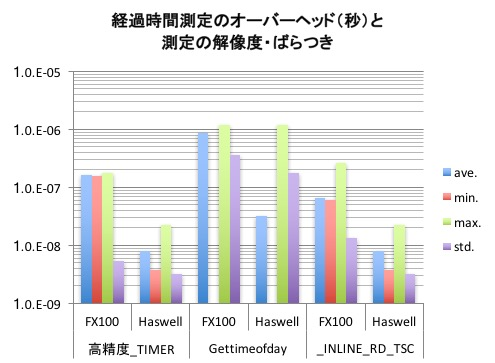
\includegraphics[width=0.45\textwidth]{figs/precise-timer.jpg}
\caption{precise-timer}
\label{fig:precise-timer}
\end{figure}



\subsection{PMlibの出力情報}
PMlibの出力として、標準出力や指定ファイルへのテキストレポート、および
汎用のトレースフォーマットであるOTF(Open Trace Format)ファイルを出力
する機能を持っている。


\subsection{関連する性能評価ツールと関連研究}


{ \color{blue} \par
各ツールにciteが必要かな
\par }

\begin{verbatim}
オープンソース性能統計ツール類 {
Gprof: 簡易機能、コンパイラに制約
Scalasca: 高機能、Score-P共通インフラ
Extrae : トレース生成
PAPI : HWPCへのアクセス
Linux perf tools : HWPCへのアクセス
}
ベンダーツール {
X86系では
Intel Vtune : X86
PGI profiler : X86
富士通プロファイラ : Sparc64系
}

それぞれに特徴があり、
ベンダー製品の性能計測・統計ツールは{
	○豊富な機能が統合化されたインタフェイス
	○パッケージの完成度が高く、インストールが容易
	○ 詳しいドキュメント、ベンダーによるサポート、安心感
	△一般に高価格で相当の習熟期間が必要
	△選択できるツールがシステム毎に制限される
}
オープンソースの性能計測・統計ツールは{
	○各ツール毎に特徴・機能が明確
	○様々なシステムへの移植可能
	○価格の心配が不要
	△ユーザーインタフェイスが個性的
	△ものによりインストール・利用がそれなりに大変
}
\end{verbatim}

既存ツールはほぼ全てが
サンプリングあるいはトレーシングによる測定で、性能の根拠は
HWPC情報を利用している

\section{PMlibを用いた性能測定と分析例}


\subsection{PMlibを用いた性能測定方法}

{ \color{blue}
発表スライドではCCA/EBT、OTF、HWPC(PAPI)を説明。そこに力点をおくとよい\\
}

(3)PMlibでどのような分析ができるか
・演算の種類毎に処理の「重たさ」を評価
・・浮動小数点四則演算、平方根や三角関数などの基本計算
・・・ー>コンピュータが見かけ上発揮する実行性能と、実際の数値計算性能との定量的な比較ができる
・・・ー>アプリのコーディングの指針に使える
・HWPCベースでのアーキテクチャの有効利用状況
・・使いやすい用にグループ化した統計出力
・・SSE/AVX系命令の実行比率
・・・ー>SIMD機構の有効利用の確認
・・キャッシュヒット率
・・・ー>コンパイラがどれだけ賢くコンピュータの能力を引き出しているか評価ができる
・・・ー>コンパイラオプションの選択、指示行の指定などで、どのような効果が現れるか

・ピーク性能に対する実効性能比を裏付けてみる

{ \color{blue}
Skylakeの例で示すといい\\
ルーフラインモデルを示し、実測との比較を見るとよい\\
}

以下の\lstlistingname \ref{listing1}はPMlib APIを利用するFortranソースプログラムの例である。

%lstlistingのcaptionは思い通りについてくれないので手を抜いてみるw
%\begin{lstlisting}[caption={FortranプログラムへのPMlib組み込み例},label={listing1},captionpos=b]
%	\begin{lstlisting}[caption=strangeeffect,captionpos=t]
\begin{lstlisting}[caption={\hfill},label={listing1},captionpos=t]
program main
call f_pm_initialize (nWatch)
call f_pm_setproperties ("Koko!" icalc, iexcl)
call f_pm_start ("Koko!")
call mykernel (msize,n,a,b,c)
call f_pm_stop ("Koko!", fops, ncall)
call f_pm_print ("", isort)
call f_pm_printdetail ("", ilegend, isort)
end
\end{lstlisting}

\subsection{PMlibを用いた測定例}

\subsubsection{性能測定の条件}

測定には以下のHPCシステムを用いた。
\begin{itemize}
{
%	\setlength{\itemsep}{-5pt}
%	\setlength{\topsep}{2mm}
\item Intel Skylake CPU搭載サーバ
\item 富士通prime HPC FX100
}
\end{itemize}

これらプラットフォームの主にCPU部分についての性能諸元を
表\ref{tab:server-config}に示す。

%\tiny
%\footnotesize
%\small
\begin{table}[tb]
\scriptsize
\caption{サーバの構成と最大性能(主にCPU部分)}
\label{tab:server-config}
\footnotesize
\begin{tabular}{l|c|c} \hline
\scriptsize
system			&	FX100	&	Skylake	\\ \hline
CPU				&	SPARC64 VIIIifx	&	Gold 6148	\\ \hline
core GHz		&	1.975	&	2.4	\\ \hline
core Gflops	&	31.6	&	〜30	\\ \hline
L1\$ size (D,I)		&	64KB, 64KB	&	32KB, 32KB	\\ \hline
L1D\$ BW GB/s	&	140/R+70/W	&	154/R + 77/W	\\ \hline
\$ Linesize 	&	256B	&	64B	\\ \hline
L2\$ size		&	-	&	1MB	\\ \hline
L2\$ BW GB/s/core	&	-	&	154 ( ~70)	\\ \hline
LL\$ size		&	12MB	&	28MB(1.4MB/c)	\\ \hline
LL\$ BW GB/s/core	&	70/R+35/W	&	77 ( ~43)	\\ \hline
Memory			&	HMC(8x16Ls)	&	DDR4-2666	\\ \hline
Mem GB/s/[CMGcpu]	&	120/R+120/W	&	128	\\ \hline
\#cores/[CMGcpu]	&	16	&	20	\\ \hline
\end{tabular}
\end{table}

性能測定には以下のプログラムを用いた
\begin{itemize}
\item{基本的な演算}
\item{STREAM}
\end{itemize}


\subsubsection{基本的な演算性能の評価}

基本的な演算カーネル例として以下の様な、四則演算、平方根、3平方逆数
の配列計算を評価する。

基本的な演算カーネル例のソース:\lstlistingname \ref{listing2}

%	\begin{lstlisting}[label={listing2},captionpos=t]
\begin{lstlisting}[caption={\hfill},label={listing2},captionpos=t]
subroutine sub_add(a,b,c,n)
real*8 a(n), b(n), c(n)  
do i=1,n
c(i)=a(i)+b(i)
end do
return

subroutine sub_mult(a,b,c,n)
c(i)=a(i)*b(i) ! 計算式以外は同様

subroutine sub_fma(a,b,c,n)
c(i)=a(i)+b(i)*d ! 計算式以外は同様

subroutine sub_divide(a,b,c,n)
c(i)=b(i)/a(i) ! 計算式以外は同様

subroutine sub_sqrt(a,b,c,n)
c(i)=sqrt(a(i)) ! 計算式以外は同様

subroutine sub_mix(a,b,c,n)
c(i)=1.0/sqrt(a(i)**2+b(i)**2) ! 他同様

\end{lstlisting}

測定したHPCシステムのOSはjitter freeではないので、以下の方法により
測定時間のフィルタリングを行った。

ソース \lstlistingname \ref{listing2} の各
サブルーチンを1000回呼び出す中間ループ、およびその中間ループを
さらに10回反復する最外側ループを設ける。
\begin{itemize}
{
\item {各スレッドがサブルーチンを1000回呼び出す中間ループを実行し、
		その時間を測定する。}
\item {上の測定を10回繰り返して、標準偏差1σの範囲だけを採用する。}
\item {採用した測定値の平均値をスレッドの代表値とする}
\item {全スレッドの代表値の内、最小値をプロット用に採用}
}
\end{itemize}






\subsubsection{STREAM性能の評価}
STREAMベンチマーク\cite{stream:1995}
はコンピュータシステムのメモリバンド幅を測定するためのツールとして広く用いられている。
STREAMは変数配列の積和算(TRIAD)など、メモリread/write処理が主要な負荷となる
計算式の性能をアプリケーションプログラムレベルで測定出力する。
したがってその結果は「計算科学的観点」で評価された性能である。
このSTREAMプログラムを「システム評価的観点」で評価するとかなり様相が異なって来る。

まずSTREAMをSkylakeサーバ上で実行した場合の出力結果を示す。
Intelコンパイラのデフォルトオプションを用いている。
STREAM FortranプログラムOpenMPスレッド並列版を
1CPU上で8スレッド実行した場合、20スレッド実行した場合について示す。


Skylakeサーバ
されたHWPCベースでの
PMlibを用いて
メモリ階層での実測イベントベースによるデータ移動の状況を示す。
図



Intelコンパイラにはオプションが多数あり、中でも特にメモリバンド幅に関係が深いと
思われる以下のオプションを組み合わせて比較した結果を
図\ref{fig:stream-ivy-compact-1cpux8} に示す。\\
{\color{blue}この図は仮置きでIvybridgeの結果。Skylakeの結果と差し替えること。}

\begin{figure}[tb]
\centering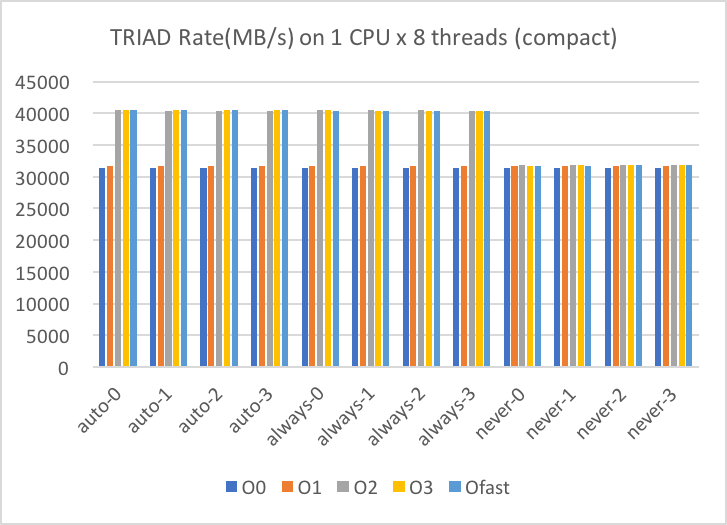
\includegraphics[width=0.45\textwidth]{figs/stream-ivy-compact-1cpux8.png}
\caption{stream-ivy-compact-1cpux8}
\label{fig:stream-ivy-compact-1cpux8}
\end{figure}


配列のファーストタッチなどデータの局所性確保、スレッドのコア固定など
を注意深く行うと、ノードに搭載された4CPUの全コアを使用した場合でも
同じような傾向の結果が得られる。
図\ref{fig:stream-ivy-scatter-4cpux8} に示す。\\

\begin{figure}[tb]
\centering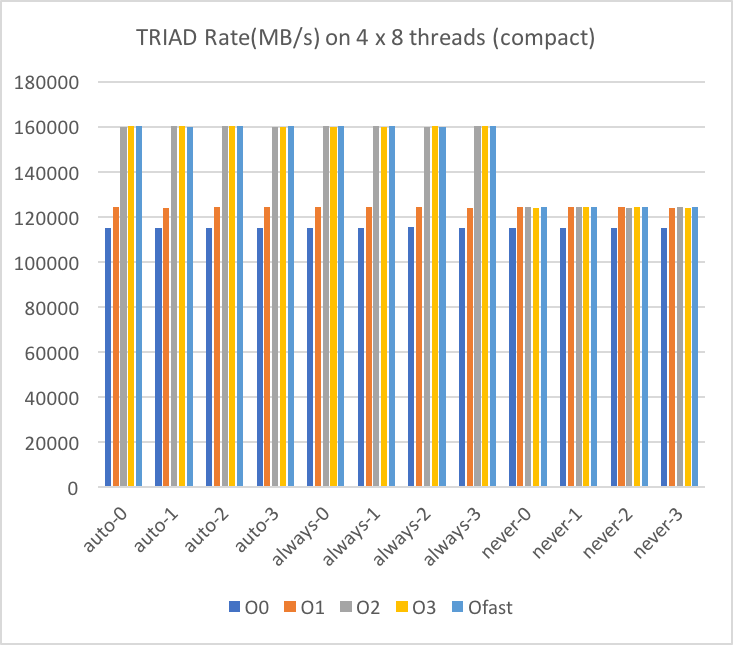
\includegraphics[width=0.45\textwidth]{figs/stream-ivy-scatter-4cpux8.png}
\caption{stream-ivy-scatter-4cpux8}
\label{fig:stream-ivy-scatter-4cpux8}
\end{figure}

これに対してアプリケーションのスレッド並列度が低い場合は様子が変わり、
例えばCPUあたり2スレッド(2コア)が実行されると
図\ref{fig:stream-ivy-scatter-4cpux2} の様になる。\\

\begin{figure}[tb]
\centering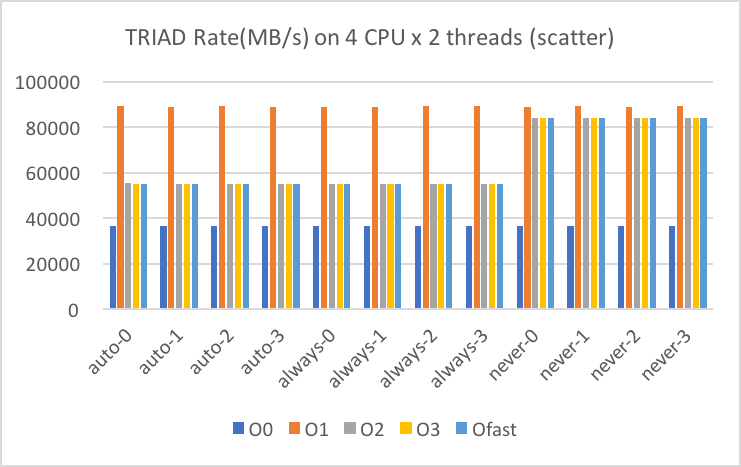
\includegraphics[width=0.45\textwidth]{figs/stream-ivy-scatter-4cpux2.png}
\caption{stream-ivy-scatter-4cpux2}
\label{fig:stream-ivy-scatter-4cpux2}
\end{figure}

図\ref{fig:stream-ivy-compact-1cpux8} と
図\ref{fig:stream-ivy-scatter-4cpux2} と
とでPMlibが出力するHWPC Cache関係の数値を比較すると***
が読み取れる。


{ \color{blue} \par
note STREAM:Intel compilerでCache Eviction Levelオプションの指定効果はほとんど
なかった
} \par


\section{謝辞}
京補助金についての謝辞

\bibliographystyle{jplain}
\bibliography{main}
\end{document}

